\documentclass[../main.tex]{subfiles}
\graphicspath{
    {"../img/"}
    {"img/"}
}
\begin{document}

$\frac{\partial H}{\partial r} = \left .\frac{\partial f}{\partial x} \right |_{\substack{x=\Psi_1(r,\varphi),\\y=\Psi_2(r,\varphi)}} \frac{\partial \Psi_1}{\partial r} + \frac{\partial f}{\partial y} \frac{\partial \Psi_2}{\partial r}\\
\frac{\partial H}{\partial \varphi} = \frac{\partial f}{\partial x} \frac{\partial \Psi_1}{\partial y} + \frac{\partial f}{\partial y} \frac{\partial \Psi_2}{\partial \varphi}$


\begin{large}
        Konwencja z ćwiczeń z fizyki:
\end{large}

$H(r,\varphi) = (f \circ \Psi)(r,\varphi)\\
H(r,\varphi)=f(r,\varphi)$
\begin{align*}&\Psi_1(r,\varphi)=x(r,\varphi)\\
              &\Psi_2(r,\varphi)=y(r,\varphi)\end{align*}
$\frac{\partial f}{\partial r} = \frac{\partial f}{\partial x} \frac{\partial x}{\partial r} + \frac{\partial f}{\partial y} \frac{\partial y}{\partial r}\\
\frac{\partial f}{\partial \varphi} = \frac{\partial f}{\partial x} \frac{\partial x}{\partial \varphi} + \frac{\partial f}{\partial y} \frac{\partial y}{\partial \varphi}$

\begin{przyklad}

\end{przyklad}
$$f(x,y):\mathbb{R}^2 \to \mathbb{R},\quad
\left [ \begin{matrix}
x=r\cos{\varphi}\\
y=r\sin{\varphi}\end{matrix}\right ]$$
$$\frac{\partial f}{\partial r} = \cos{\varphi} \frac{\partial f}{\partial x} + \sin{\varphi} \frac{\partial f}{\partial y},\quad
\frac{\partial f}{\partial \varphi} = -r\sin{\varphi} \frac{\partial f}{\partial x} + r\cos{\varphi} \frac{\partial f}{\partial y}$$
$$f(x,y):\mathbb{R}^2 \to \mathbb{R},\quad
f'= \Big [ \frac{\partial f}{\partial x} , \frac{\partial f}{\partial y} \Big ]$$

\begin{large}
    Interpretacja geometryczna
\end{large}
Rozważmy zbiór $$P_c = \{(x,y)\in \mathbb{R}^2 : f(x,y) = c \} \text{ np. } f(x,y) = x^2 + y^2 : P_c = \{(x,y)\in\mathbb{R}^2 : x^2+y^2 = c \}$$

Załóżmy, że $f(x,y)$ - taka, że $P_c$ - można sparametryzować jako $$~ \varphi(t) = \left [ \begin{matrix}
x(t)\\
y(t)\end{matrix}\right ], t\in D\text{, to znaczy, że }P_c = \{(x(t),y(t)), t\in D\}$$

\begin{przyklad}

\end{przyklad}
Niech $\varphi(t) = \left [ \begin{matrix}

\cos{t}\\
\sin{t}\end{matrix}\right ]$. Wtedy $P_c = \{(c\cos{t},c\sin{t});t\in[0,2\pi]\}$

$f(x(t),y(t)) = c \quad\underset{t\in D}{\forall}$ - powierzchnie ekwipotencjalne

$$\Big [ \frac{\partial f}{\partial x} , \frac{\partial f}{\partial y} \Big ] \left [ \begin{matrix}
x'(t)\\
    y'(t)\end{matrix}\right ] = 0, \Big [ 2x, 2y \Big ] \left [ \begin{matrix}
-c\sin{t}\\
c\cos{t}\end{matrix}\right ] = 0$$

\pagebreak

\begin{figure}
    \centering
    \includegraphics[width=0.7\textwidth]{fig_3}
    \caption{Trajektoria kluki}
    \label{fig:kulka}
\end{figure}

\begin{figure}
    \centering
    \includegraphics[width=0.7\textwidth]{fig_4}
    \caption{Powierzchnia ekwipotencjalna I}
    \label{fig:ekwiI}
\end{figure}

\begin{figure}
    \centering
    \includegraphics[width=0.7\textwidth]{fig_5}
    \caption{Powierzchnia ekwipotencjalna II}
    \label{fig:ekwiII}
\end{figure}

\pagebreak


\begin{definicja}
    Pochodna mieszana
\end{definicja}
$$f(x,y) = x^2y^3, \quad \frac{\partial f}{\partial x} = 2xy^3, \frac{\partial f}{\partial y} = 3x^2y^2,\quad
\frac{\partial }{\partial x} \big (\frac{\partial f}{\partial x} \big ) = 2y^3,\quad
\frac{\partial }{\partial y} \big (\frac{\partial f}{\partial y} \big ) = 6x^2y$$


$$\frac{\partial^2 f}{\partial x \partial y} = 6xy^2 \quad \frac{\partial^2 f}{\partial y \partial x} = 6xy^2$$
\textbf{Przypadek???}

\begin{tw}
Niech $f: \mathcal{O}\to\mathbb{R}, \mathcal{O}\subset \mathbb{R}^n$, otwarty i $f\in\mathcal{C}^2(\mathcal{O})$, wówczas
$$\frac{\partial^2 f}{\partial x^i \partial x^j} = \frac{\partial^2 f}{\partial x^j \partial x^i}; i,j=1,\dots,n$$
\end{tw}

\begin{dowod}
    Dowód dla $n=2$
\end{dowod}
Niech $w(x,y) = f(x+h,y+k) - f(x+h,y) - f(x,y+k) + f(x,y)$\\
$\varphi(x) = f(x,y+k) - f(x,y)$\\
wówczas
\begin{align*}
    &w=\varphi(x+h) - \varphi(x) = \frac{\partial \varphi}{\partial x} (\xi)h = \\
&=\Big [ \frac{\partial f}{\partial x} (\xi, y+k) - \frac{\partial f}{\partial x} (\xi, y) \Big ]h = \frac{\partial }{\partial y} \Big ( \frac{\partial f}{\partial x} (\xi,\eta) \Big ) hk
,\\
    & \text{gdzie }x<\xi<x+h,\quad y<\eta<y+k
\end{align*}

Niech $\Psi(y)=f(x+h,y)-f(x,y)\\
w(x,y) = \Psi(y+k) - \Psi(y) = \frac{\partial \Psi}{\partial y} (\eta_1)k = \Big [\frac{\partial f}{\partial y} (x+h,\eta_1) - \frac{\partial f}{\partial y} (x,\eta_1) \Big ] k = \frac{\partial }{\partial x} \Big ( \frac{\partial f}{\partial y} (\xi,\eta) \Big ) kh$, czyli $\underset{\xi\in]x,x+h[}{\exists},\quad \xi_1\in]x,x+h[,\quad \eta\in]y,y+k[,\quad \eta_1\in]y,y+k[ \quad (y<\eta_1<y+k)$

Jeżeli $h\to 0\\
\bigg ( \frac{\partial^2 f}{\partial y \partial x} (\xi,\eta) = \frac{\partial^2 f}{\partial x \partial y} (\xi_1,\eta_1) \bigg )$

to $\xi \to x, \xi_1 \to x, \eta \to y, \eta_1 \to y$, czyli:
$$\frac{\partial^2 f}{\partial y \partial x} (x,y) = \frac{\partial^2 f}{\partial x \partial y} (x,y) $$
Jeżeli każda z tych wielkości jest ciągła $\Box$

\begin{large}
    Wzór Taylora
\end{large}
Niech $f: \mathcal{O}\to\mathbb{R}, \mathcal{O}\subset \mathbb{R}^n$ - otwarty\\
$\varphi(t) = f(x_0+th), h\in \mathbb{R}^n, t\in[0,1]$

\vspace{0.5cm}
Dla $h=\left [ \begin{matrix}
h^1\\
\vdots\\
h^n\end{matrix}\right ] ,
x_0 = \left [ \begin{matrix}
x_0^1\\
\vdots\\
x_0^n\end{matrix}\right ],
\varphi(t) = f(x_0^1+th^1,x_0^2+th^2,\dots,x_0^n+th^n)$
\vspace{0.5cm}

$\frac{\partial \varphi}{\partial t} = \left .\frac{\partial f}{\partial x^1} \right |_{x=x_0+th} h_1 + \left .\frac{\partial f}{\partial x^2} \right |_{x=x_0+th} h_2 + \dots + \left .\frac{\partial f}{\partial x^n} \right |_{x=x_0+th} h_n = \left .\sum_{i=1}^n \frac{\partial f}{\partial x^i} \right |_{x_0+th}h_i$

$\frac{\partial^2 \varphi}{\partial t^2} = \left .\sum_{j=1}^n \sum_{i=1}^n \frac{\partial f}{\partial x^i \partial x^j} \right |_{x_0+th} h_j h_i$

$\vdots$

$\frac{\partial^k \varphi}{\partial t^k} = \sum_{i^1,\dots,i^k}^n \frac{\partial^{(k)} f}{\partial x^{i_{1}} \dots \partial x^{i}} h_{i_1}\dots h_{i_k}$

$\varphi(t) = \varphi(0) = \varphi'(0)(t-0)+\frac{\varphi''(0)}{2!}(t-0)^2+\dots+\frac{\varphi^k(0)}{k}(t-0)^k + r(\dots)$

Czyli:
$$\varphi(1)-\varphi(0) = \varphi'(0)+\frac{\varphi''(0)}{2!} + \frac{\varphi'''(0)}{3!} + \dots + \frac{\varphi^k(0)}{k!}+r(\dots)$$

$$f(x_0+h)-f(x_0)=\sum_{i=1}^n \frac{\partial f}{\partial x^i} (x_0) h_i + \frac{1}{2!} \sum_{i,j=1}^n \frac{\partial^2 f}{\partial x^i \partial x^j} (x_0)h_ih_j + \dots \dots \Box$$

\end{document}
